% The entire content of this work (including the source code
% for TeX files and the generated PDF documents) by 
% Hongxiang Chen (nicknamed we.taper, or just Taper) is
% licensed under a 
% Creative Commons Attribution-NonCommercial-ShareAlike 4.0 
% International License (Link to the complete license text:
% http://creativecommons.org/licenses/by-nc-sa/4.0/).
\documentclass{article}

\usepackage{float}  % For H in figures
\usepackage{amsmath} % For math
\usepackage{amssymb}
\usepackage{mathrsfs}
% Followings are for the special character: differential "d".
\newcommand*\diff{\mathop{}\!\mathrm{d}}
\newcommand*\Diff[1]{\mathop{}\!\mathrm{d^#1}}
\numberwithin{equation}{subsection} % have the enumeration go to the subsection level.
                  % See:https://en.wikibooks.org/wiki/LaTeX/Advanced_Mathematics
\usepackage{graphicx}   % need for figures
\usepackage{cite} % need for bibligraphy.
\usepackage[unicode]{hyperref}  % make every cite a link
\usepackage{CJKutf8} % For Chinese characters
\usepackage{fancyref} % For easy adding figure,equation etc in reference. Use \fref or \Fref instead of \ref
\usepackage{braket} %http://tex.stackexchange.com/questions/214728/braket-notation-in-latex

% Following is for theorems etc environments
% http://tex.stackexchange.com/questions/45817/theorem-definition-lemma-problem-numbering && https://en.wikibooks.org/wiki/LaTeX/Theorems
\usepackage{amsthm}
\newtheorem{defi}{Definition}[section]
\newtheorem{thm}{Theorem}[section]
\newtheorem{lemma}{Lemma}[section]
\newtheorem{remark}{Remark}[section]
\newtheorem{prop}{Proposition}[section]
\newtheorem{coro}{Corollary}[section]
\theoremstyle{definition}
\newtheorem{ex}{Example}[section]

% A list of nomenclatures.
\usepackage{nomencl}
\makenomenclature

% For better indices
\usepackage{tensor}
% ANCHOR

% For highlighting
\usepackage{xcolor,soul}

% For category graphs
\usepackage[all]{xy}

\title{Miscellaneous notes for D. Huybrechts's Complex Geometry}
\date{\today}
\author{Taper}


\begin{document}


\maketitle
\abstract{
Miscellaneous notes for D. Huybrechts's book \textit{Introduction
to Complex Geometry}, include some homeworks done.
}
\tableofcontents
\section{The structure of almost complex structures on \texorpdfstring{$\mathbb{R}^{4}$}{}
  (exercise 1.2.1)}
\label{sec:The_structure_of_almost_complex_structures_on_R2n}
In exercise 1.2.1, it says that the set of all compatible almost complex
structures on a euclidean space of dimension $4$, is two copies of $S^2$.

To show it, I tried first a straight calculation. Assuming the almost
complex structure $I= (a_{ij})$. Then we have:
\begin{figure}[H]
  \centering
  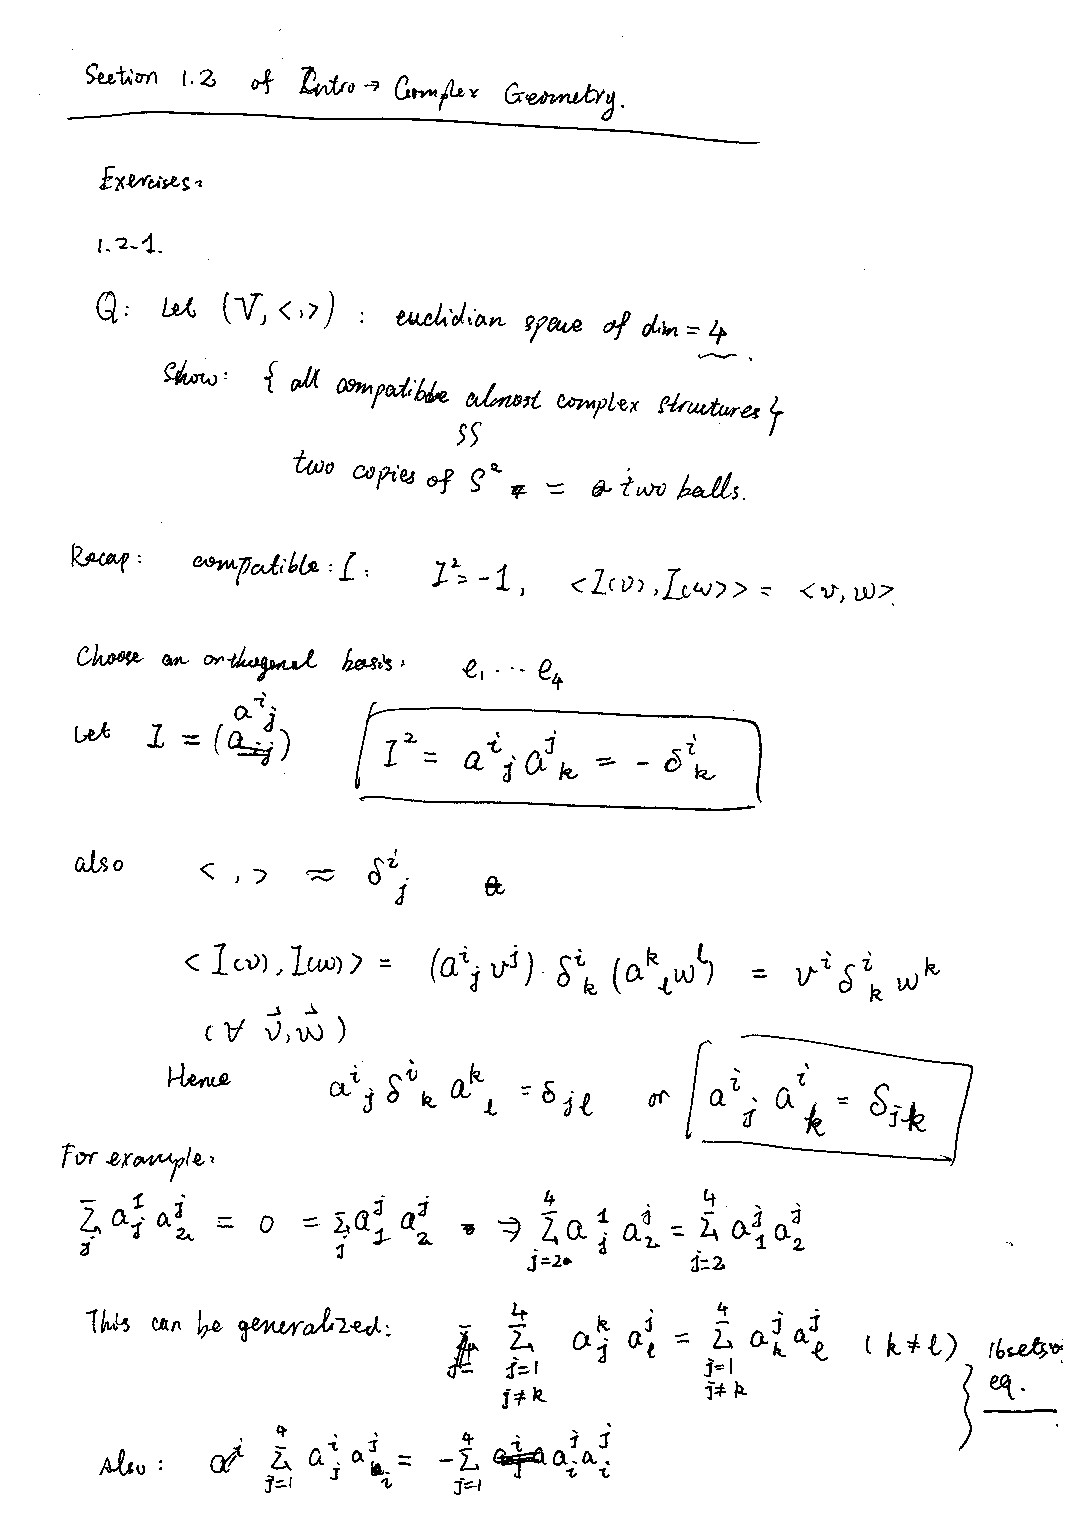
\includegraphics[scale=0.70]{pdfs/draft_20160908.pdf}
  \caption{Draft}
\end{figure}

Then I discover this too hard to work, because too many equations are
involed, and none of them could be eliminiated by other. Meanwhile, I
found a post in Math.SE about this \cite{math.se_1}. Here are several
important concepts for understanding that post.

    \subsection{Understand \texorpdfstring{ 
                    $\frac{GL(2n,\mathbb{R})}
                        {GL(n,\mathbb{C})}$
                            }{}
                }
    \label{sec:Understand_GL(2n,R)/GL(n,C)}

        \subsubsection{Why \texorpdfstring{$M_n = \frac{GL(2n,\mathbb{R})}
            {GL(n,\mathbb{C})}$}{}}

        This is a note of my question on Math.SE\cite{math.se_3}, which
        explains that we can identify the set of almost complex structures
        with $\frac{GL(2n,\mathbb{R})}{GL(n,\mathbb{C})}$.

        First, I try to do it when $n=1$. I inject a complex number 
        $a+bi$ by
        identify it with $a\mathbb{I}+b\mathbb{J}$, where $\mathbb{I}$ 
        is the identify matrix and $\mathbb{J}$ is
        $ \left(
        \begin{array}{cc}
         0 & -1 \\
         1 & 0 \\
        \end{array}
        \right) $. I take one set of basis of 
        $\mathrm{GL}(2,\mathbb{R})$ as:
        $$
        \left(
        \begin{array}{cc}
         1 & 0 \\
         0 & 1 \\
        \end{array}
        \right),\left(
        \begin{array}{cc}
         0 & -1 \\
         1 & 0 \\
        \end{array}
        \right),\left(
        \begin{array}{cc}
         0 & 0 \\
         1 & 0 \\
        \end{array}
        \right),\left(
        \begin{array}{cc}
         0 & 0 \\
         0 & 1 \\
        \end{array}
        \right)
        $$

        (I think this is a basis because the following matrix is 
        non-singular:
        $$
        \left(
        \begin{array}{cccc}
         1 & 0 & 0 & 0 \\
         0 & -1 & 0 & 0 \\
         0 & 1 & 1 & 0 \\
         1 & 0 & 0 & 1 \\
        \end{array}
        \right)
        $$)
        Then the $\frac{\mathrm{GL}(2n,\mathbb{R})}{\mathrm{GL}
        (n,\mathbb{C})}$ becomes equivalent classes represented by 
        $$
        \left(
        \begin{array}{cc}
         0 & 0 \\
         c & d \\
        \end{array}
        \right)
        $$

        However, I don't know how to link this with an almost complex 
        structure.  

        I have a feeling that I might have been in the wrong direction. 
        It was pointed out that $\mathrm{GL}(2n,\mathbb{R})$ is not
        even a vector space. So what I did is in fact nonsense.
        
        Below is one correct answer I got:

        \begin{center}\noindent\rule{8cm}{0.4pt}\end{center}
        
        An almost-complex structure is a matrix $J$ such that $J^2 = -I$
        is the negative identity. As you said, one example of such a 
        matrix $J$ is $$\begin{pmatrix} 0 & I \\ -I & 0 \end{pmatrix}.$$

        Interpreting $GL(n,\mathbb{C})$ as a subgroup of 
        $GL(2n;\mathbb{R})$ depends on having fixed such an 
        almost-complex structure. Once we have a matrix $J$, we can call 
        a matrix $A \in GL(2n;\mathbb{R})$ complex-linear if it commutes 
        with $J$, i.e. $AJA^{-1} = J.$

        (The idea is that $\mathbb{C}$-linear maps $T$ are just real 
        linear maps with the additional property that $T(iv) = i T(v)$
        for all vectors $v$)

        Given any matrix $A \in GL(2n;\mathbb{R})$, we get another 
        almost-complex structure $AJA^{-1}$. This is the same 
        almost-complex structure $J$ if and only if 
        $A \in GL(n;\mathbb{C}).$ On the other hand, all almost-complex 
        structures are similar (although it may take some work to be 
        convincing that they are similar over $\mathbb{R}$ and not 
        only $\mathbb{C}$) since they are diagonalizable with the same 
        eigenvalues $\pm i$. That gives you a bijection 
        $$
            GL(2n;\mathbb{R}) / GL(n;\mathbb{C}) \longrightarrow 
            \{\mathrm{almost}-\mathrm{complex}\; 
            \mathrm{structures}\}
        $$ 
        under which a class $A \cdot GL(n;\mathbb{C})$ corresponds 
        to the almost-complex structure $AJA^{-1}.$

        \begin{center}\noindent\rule{8cm}{0.4pt}\end{center}

        I questioned him:
        \begin{enumerate}
            \item Why $AJA^{-1}$ is the same almost-complex structure 
                $J$ if and only if $A\in \mathrm{GL}(n;\mathbb{C})$. 
            \item Why all almost-complex structures are similar over 
                $\mathbb{R}$.
        \end{enumerate}
        He responsed that:
        \begin{enumerate}
            \item is the definition of $\mathrm{GL}(n;\mathbb{C})$
                as matrices $A$ with $AJA^{-1}=J$.
            \item comes from the fact that any real matrices that are 
                similar over $\mathbb{C}$ are already similar over 
                $\mathbb{R}$. This isn't trivial but it has been asked 
                and answered many times on this site: here is one 
                reference \cite{math.se_4}.
        \end{enumerate}

        Inside that reference, the following theorem is proved:

        \begin{thm}
            Let $E$ be a field, let $F$ be a subfield, and let $A$ and
            $B$ be $nxn$ matrices with coefficients in $F$. If $A$ and
            $B$ are similar over $E$, they are similar over $F$.
        \end{thm}

        However, I still have doubts about the following question:
        For $A\in \mathrm{GL}(2n,\mathbb{R})$, if $AJA^{-1}=J$, can we
        conlude that $A$ is inside $\mathrm{GL}(n,\mathbb{C})$?

        The following is my solution:
        \begin{lemma}
            There exists a injection $\phi$ of $\mathrm{GL}(n,\mathbb{C})
            \hookrightarrow \mathrm{GL}(2n,\mathbb{R})$ such that:
            \begin{align}
                \phi(i B)= \phi(i)\phi(B)
            \end{align}
            for any $B\in \mathrm{GL}(n,\mathbb{C})$. Also, for any
            $A\in \mathrm{GL}(2n,\mathbb{R})$ we have $AJA^{-1}=J$
            if and only if $A\in \mathrm{Im}(\phi)$, where $J\equiv\phi(i)$.
        \end{lemma}
        
        \begin{proof}
            The $\phi$ is construct as follows. Let 
            $J_0=\left( \begin{array}{cc}
                 0 & -1 \\
            1 & 0 \\ \end{array} \right)$, define $H(x+iy)$ for
            $x,y\in \mathbb{R}$ as
            \begin{align}
                H(x+iy) = x I + y J
            \end{align}
            Then:
            \begin{align}
                \phi(A)_{ij} \equiv H(a_{ij})
            \end{align}
            Then:
            \begin{align}
                \phi(i) = \left( \begin{array}{ccc}
                     J & 0 & 0 \\
                     0 & \text{...} & 0 \\
                     0 & 0 & J \\
                    \end{array} \right)
            \end{align}
            By direct simple calculation (remember to use the technique
            of block multiplication), we have:
            $\phi(i B)= \phi(i)\phi(B)$.
            for any $B\in \mathrm{GL}(n,\mathbb{C})$. This also shows 
            $BJB^{-1}=J$, since $iB=Bi$.
            
            To prove the converse, we see that the following matrices forms
            a basis of $2x2$ real matrices:
            $$ \left( \begin{array}{cc}
             1 & 0 \\
             0 & 1 \\ \end{array}
            \right),\left( \begin{array}{cc}
             0 & -1 \\
             1 & 0 \\ \end{array}
            \right),\left( \begin{array}{cc}
             0 & 0 \\
             1 & 0 \\ \end{array}
            \right),\left( \begin{array}{cc}
             0 & 0 \\
             0 & 1 \\ \end{array} \right) $$
            They are denoted, from left to right as $I,J_0,K,L$.
            \marginpar{Fun fact: $[K,J_0]=\sigma_z\;,[L,J_0]=\sigma_x$, the
            pauli matrices!}
            Let any $A\in \mathrm{GL}(2n,\mathbb{R})$, we can partition $A$
            into a matrix of $2x2$ matrices $(a_{ij})$. Each matrix can
            the be expressed as $a_{ij}=x_{ij}I+y_{ij}J_0+z_{ij}K+t_{ij}L$.
            Then if $AJA^{-1}=J$, by direct calculation we find:
            $$ (z_{ij}K+t_{ij}L)J_0=J_0(z_{ij}K+t_{ij}L)$$
            then also by direct calculation, it can be easily found that
            $z_{ij}=t_{ij}=0$. Hence $A\in \mathrm{Im}(\phi)$.
        \end{proof}
        
        \subsubsection{Why \texorpdfstring{
                $GL(n, \mathbb{C}) \hookrightarrow GL^+(2n,\mathbb{R})$
                }{}
            }
        
        To understand that post \cite{math.se_1}, I also read this
        \cite{math.se_2}. In it, it asks how to prove that 
        \begin{align}
            \label{eq:sec.1.1.2_why_glnc_injectInto_positive_comp}
            GL(n, \mathbb{C}) \hookrightarrow GL^+(2n,\mathbb{R})
        \end{align}
        for any $n$. The questioner gives the intuition for this fact:
        \begin{center}\noindent\rule{8cm}{0.4pt}\end{center}
        
        \begin{quote}
            how about since as Lie groups, $GL(n,\mathbb{C}) 
            \subset GL(2n, \mathbb{R})$ and $GL(n,\mathbb{C})$ is connected 
            but $GL(2n, \mathbb{R})$ has two connected components, one for 
            positive determinant and one for negative determinant? And the 
            identity has positive determinant, so it must lie in that 
            component.
        \end{quote}
        \begin{center}\noindent\rule{8cm}{0.4pt}\end{center}
        
        Someone answered that question: 

        \begin{center}\noindent\rule{8cm}{0.4pt}\end{center}
        
        \begin{quote}
            The claim is: If $V$ is an $n$-dimensional complex vector space with underlying $2n$-dimensional real vector space $W$, then the canonical group monomorphism $\mathrm{GL}(V) \to \mathrm{GL}(W)$ lands inside $\mathrm{GL}^+(W)=\{f \in \mathrm{GL}(W) : \det(f)>0\}$.  The purpose of this abstract reformulation is that we may use operations on vector spaces in order to simplify the problem: If $V'$ is another finite-dimensional complex vector space with underlying real vector space $W'$, the diagram

            \begin{align}
              \begin{array}{ccc} 
                \mathrm{GL}(V) \times \mathrm{GL}(V') & \rightarrow & \mathrm{GL}(W) \times \mathrm{GL}(W') \\
                \downarrow & & \downarrow \\ 
                \mathrm{GL}(V \oplus V') & \rightarrow & \mathrm{GL}(W \oplus W') 
              \end{array}
            \end{align}

            commutes, and the image of $\mathrm{GL}^+(W) \times \mathrm{GL}^+(W')$  is contained in $\mathrm{GL}^+(W \oplus W')$. Therefore, if some element in $\mathrm{GL}(V \oplus V')$ lies in the image of $\mathrm{GL}(V) \times \mathrm{GL}(V')$, it suffices to consider the components. Combining this with the fact that $\mathrm{GL}(V)$ is generated by \href{https://en.wikipedia.org/wiki/Elementary_matrix}{elementary matrices} (after chosing a basis of $V$), we may reduce the whole problem to the following three types of matrices:

            - the $1 \times 1$-matrices $(\lambda)$,

            - the $2 \times 2$-matrices $\begin{pmatrix} 1 & 0 \\ \lambda & 1 \end{pmatrix}$,

            - and the $2 \times 2$-matrix $\begin{pmatrix} 0 & 1 \\ 1 & 0 \end{pmatrix}$.

            Write $\lambda=a+ib$ with $(a,b) \in \mathbb{R}^2 \setminus \{(0,0)\}$. Then, the complex $1 \times 1$-matrix $(\lambda)$ becomes the real $2 \times 2$-matrix $\begin{pmatrix} a & -b \\ b & a \end{pmatrix}$, which has determinant $a^2+b^2 > 0$. The complex $2 \times 2$-matrix $\begin{pmatrix} 1 & 0 \\ \lambda & 1 \end{pmatrix}$ becomes the real $4 \times 4$-matrix
            $\begin{pmatrix}
            1 & 0 & 0 & 0 \\
            0 & 1 & 0 & 0 \\
            a & -b & 1 & 0 \\
            b & a & 0 & 1 \end{pmatrix}$, 
            which has determinant $1$. Finally, the complex $2 \times 2$-matrix  $\begin{pmatrix} 0 & 1 \\ 1 & 0 \end{pmatrix}$ becomes the real $4 \times 4$-matrix $\begin{pmatrix} 0 & 0 & 1 & 0 \\ 0 & 0 & 0 & 1\\ 1 & 0 & 0 & 0 \\ 0 & 1 & 0 & 0 \end{pmatrix}$, which has determinant $1$.

        \end{quote}
        \begin{center}\noindent\rule{8cm}{0.4pt}\end{center}
        
        However, this proof is not complete because, to build the proof from 
        $\mathbb{R}^2$ to $\mathbb{R}^{2n}$, it requries, in his argument,
        that any element in $\mathrm{GL}(V\oplus V)$ is in the image of
        $\mathrm{GL}(V)\times \mathrm{GL}(V')$, which is not the case.

        On the other hand, it seems that this property can be proved directly
        by calculation. The following will be a notes of a paper 
        \cite{determinants_of_block_m}, which one comment mentions 
        in the Math.SE post \cite{math.se_2}.

% TODO also, this post may be useful:http://math.stackexchange.com/questions/1400917/equivalence-of-almost-complex-structures

        \subsubsection{Determinants of Block Matrices}
        \label{sec:Determinants of Block Matrices}
        
        This paper tries to prove the theorem:

        \begin{thm}
            %\label{thm:determinant_of_block_m}
            Let $R$ be a commutative subring of $\tensor[^n]{F}{^n}$,
            where $F$ is a field (or a commutative ring), and let 
            $M\in \tensor[^m]{R}{^m}$. Then 
            \begin{align}
                \text{det}_F \mathbf{M} = 
                    \text{det}_F( \text{det}_R \mathbf{M})
            \end{align}
        \end{thm}
        
        In particular, we have:
        \begin{align}
            \text{det}_F \left(
                \begin{array}{cc}
                \mathbf{A} & \mathbf{B} \\
                \mathbf{C} & \mathbf{D} \\
                \end{array}
                \right)
                = \text{det}_F (AD-BC)
        \end{align}
        Note that, that the ring being is commutative excludes some
        ambiguity. For example, when the ring $4$ is not commutative,
        then the quantity:
        
        \begin{align}
            \text{det}_F \left(
                \begin{array}{cc}
                \mathbf{A} & \mathbf{B} \\
                \mathbf{C} & \mathbf{D} \\
                \end{array}
                \right)
        \end{align}
        is not well-defined. It can be $AD-BC$, or $DA-CB$, etc.
        
        Before the proof of the main theorem, it establishes several
        facts:
        \begin{align}
            \label{eq:sec1.1.1_fact_5}
            \text{det}_F  \left(
                \begin{array}{cc}
                \mathbf{A} & \mathbf{0} \\
                \mathbf{C} & \mathbf{D} \\
                \end{array}
                \right)
                =& \text{det}_F \mathbf{A} \text{det}_F \mathbf{D}
            \\
            \label{eq:sec1.1.1_fact_6}
            \text{det}_F  \left(
                \begin{array}{cc}
                \mathbf{A} & \mathbf{B} \\
                \mathbf{0} & \mathbf{D} \\
                \end{array}
                \right)
                =& \text{det}_F \mathbf{A} \text{det}_F \mathbf{D}
            \\
            \label{eq:sec1.1.1_fact_8}
            \text{det}_F  \left(
                \begin{array}{cc}
                \mathbf{A} & \mathbf{B} \\
                \mathbf{C} & \mathbf{0} \\
                \end{array}
                \right)
                =& \text{det}_F \mathbf{-C} \text{det}_F \mathbf{B}
            \\
            \label{eq:sec1.1.1_fact_88}
            \text{det}_F \mathbf{A} \text{det}_F \mathbf{D}
            =& \text{det}_F \mathbf{I}_n \text{det}_F (\mathbf{AD})
        \end{align}

        He first builds up a seemingly simplified, but is actually
        different version of the main theorem:
        \begin{thm}
            \label{thm:sec_1.1.1_thm3}
            Let $\mathbf{A,B,C,D}\in \tensor[^n]{F}{^n}$. 
            Let $\mathbf{M}=\left(
                \begin{array}{cc}
                \mathbf{A} & \mathbf{B} \\
                \mathbf{C} & \mathbf{D} \\
                \end{array}
                \right)$.
            
            If
            $\mathbf{CD=DC}$, then,
            \begin{align}
                \text{det}_F \mathbf{M}= 
                \text{det}_F (\mathbf{AD-BC})
            \end{align}
        \end{thm}
        and similar results:
        \begin{align}
            \label{eq:sec1.1.1_thm3_similar}
            \text{if } \mathbf{AC=CA} &\text{then, }
                \text{det}_F \mathbf{M}= \text{det}_F (\mathbf{AD-CB})
            \\
            \text{if } \mathbf{BD=DB} &\text{then, }
                \text{det}_F \mathbf{M}= \text{det}_F (\mathbf{DA-BC})
            \\
            \text{if } \mathbf{AB=BA} &\text{then, }
                \text{det}_F \mathbf{M}= \text{det}_F (\mathbf{DA-CB})
        \end{align}
        These equalities can be proved easily by the following:
        \begin{align*}
            \left(
                \begin{array}{cc}
                 D & 0 \\
                 -C & i \\
                \end{array}
            \right) \left(
                \begin{array}{cc}
                 A & B \\
                 C & D \\
                \end{array}
            \right) &= \left(
                \begin{array}{cc}
                 \text{AD}-\text{BC} & B \\
                 \text{CD}-\text{DC} & D \\
                \end{array}
            \right)=\left(
                \begin{array}{cc}
                 \text{AD}-\text{BC} & B \\
                 0 & D \\
                \end{array}
            \right) \text{ when $C,D$ commutes}
            \\
            \left(
                \begin{array}{cc}
                 D & -B \\
                 0 & i \\
                \end{array}
            \right) \left(
                \begin{array}{cc}
                 A & B \\
                 C & D \\
                \end{array}
            \right) &= \left(
                \begin{array}{cc}
                 \text{DA}-\text{BC} & \text{DB}-\text{BD} \\
                 C & D \\
                \end{array}
            \right)=\left(
                \begin{array}{cc}
                 \text{DA}-\text{BC} & 0 \\
                 C & D \\
                \end{array}
            \right) \text{ when $D,B$ commutes.}
        \end{align*}

        The author also gives an illuminative explanation for why
        $$ \left( \text{det}_F \mathbf{M}- \text{det}_F (\mathbf{AD-BC}) 
            \right) \text{det}_F \mathbf{D} =0 $$
        necessarily implies:
        $$ \text{det}_F \mathbf{M}= \text{det}_F (\mathbf{AD-BC}) $$
       
        However, I am dubious about this conclusion, since I think it
        needs in addition that the polynomial ring $F[x]$ has not
        nonzero zero divisor.

        Having demonstrated the above simple case, the author continues to
        prove the main theorem. He proves by induction. He first uses:
        \begin{align}
            \left(
                \begin{array}{cc}
                 A & b \\
                 c & d \\
                \end{array}
            \right)  \left(
                \begin{array}{cc}
                 \text{dI} & 0 \\
                 -c & 1 \\
                \end{array}
            \right)=\left(
                \begin{array}{cc}
                 A_0 & b \\
                 0 & d \\
                \end{array}
            \right)
        \end{align}
        where $A,A_0\in \tensor[^{m-1}]{R}{^{m-1}}, 
        b\in \tensor[^{m-1}]{R}{}, c\in \tensor{R}{^{m-1}}, d\in R$. 
        Therefore, (let $M=
            \left(
            \begin{array}{cc}
             A & b \\
             c & d \\
            \end{array}
            \right)$)
        with similar reason mentioned before, he shows if:
        \begin{align}
            \text{det}_F \mathbf{A_0} =
              \text{det}_F \mathbf{( \text{det}_R \mathbf{A_0})}
        \end{align}
        (which is true by induction) then:
        \begin{align}
            \text{det}_F \mathbf{M} =
              \text{det}_F \mathbf{( \text{det}_R \mathbf{M})}
        \end{align}
        Proof completes.

        He also mentions a corollary:
        \begin{coro}
            Let $\mathbf{P}\in \tensor[^n]{F}{^n}$ and $\mathbf{Q}\in
            \tensor[^m]{F}{^m}$, then
            \begin{align}
                \text{det}_F (\mathbf{P\otimes Q}) =
                (\text{det}_F \mathbf{P}) ^m (\text{det}_F \mathbf{Q})^n
            \end{align}
        \end{coro}

        The proof is quite straightforward and is omitted.

        \subsubsection{Why \texorpdfstring{
                $GL(n, \mathbb{C}) \hookrightarrow GL^+(2n,\mathbb{R})$
                }{}(continued)
            }
        With above theorem, the proof of equation 
        \ref{eq:sec.1.1.2_why_glnc_injectInto_positive_comp} 
        is straight forward. Since for 
        $(a_{ij})= A\in \mathrm{GL}(n,\mathbb{C})$, it injects into
        $\mathrm{GL}(2n,\mathbb{R})$ as matrices of the form:
        \begin{align*}
            \left( \begin{array}{ccc}
             \text{...} & \text{...} & \text{...} \\
             \text{...} & H a_{\text{ij}} & \text{...} \\
             \text{...} & \text{...} & \text{...} \\
            \end{array} \right)
        \end{align*}
        where:
        \begin{align*}
            H(z\equiv x+iy)=\left( \begin{array}{cc}
                    x & -y \\
                    y & x \\
            \end{array}\right)
        \end{align*}
        Since $H(a_{ij})$ commutes with each other (proved by calculation),
        we can use the theorem in previous part to show that:
        \begin{align*}
            \mathrm{det_\mathbb{R}}(A) =
            \mathrm{det_\mathbb{R}}  (\mathrm{det_\mathbb{C}}(A))
            = \mathrm{det}_\mathbb{R}(aI+bJ)
            =\mathrm{det}\left(\begin{array}{cc}
                    a & -b\\
                    b & a\\
            \end{array}\right) \geq 0
        \end{align*}
        Notice that I have been sloopy in language, but the meaning should
        be clear.

    \subsection{Math.SE answer in \texorpdfstring{$M_2$}{} is two copies of \texorpdfstring{$S^2$}{}}

    Following is an answer\cite{math.se_set-of-almost}
    in Math.SE about this question:
    \begin{center}\noindent\rule{8cm}{0.4pt}\end{center}
    \begin{quote}
        As you noted, $M$ is *not* diffeomorphic to $S^2\coprod S^2$ for
        dimension reasons.

        On the other hand, what is true is $M$ is homotopy equivalent to $S^2
        \coprod S^2$.

        (The following argument is partly adapted from a [paper][1] of
        Montgomery)

        To see this, it's enough to show that
        $Gl^+(4,\mathbb{R})/Gl(2,\mathbb{C})$ is homotopy equivalent to $S^2$,
        where $Gl^+$ denotes those matrices of positive determinant.

        Now, consider the subgroups $U(2)\subseteq Gl(2,\mathbb{C})$ and
        $SO(4)\subseteq Gl^+(4,\mathbb{R})$.

        It's relatively well known that $Gl(2,\mathbb{C})$ is diffeomorphic to
        $U(2)\times \mathbb{R}^4$ and that $Gl^+(4,\mathbb{R})$ is diffeomorphic
        to $SO(4)\times \mathbb{R}^{10}$.  Further, in the usual inclusion
        $Gl(2,\mathbb{C})\rightarrow Gl^+(4,\mathbb{R})$, $U(2)$ becomes a
        subgroup of $SO(4)$.

        Now, the chain of subgroups $U(2)\subseteq SO(4)\subseteq
        Gl^+(4,\mathbb{R})$ gives rise to a homogeneous fibration
        $$SO(4)/U(2)\rightarrow Gl^+(4,\mathbb{R})/U(2)\rightarrow
        Gl^+(4,\mathbb{R})/SO(4).$$  \hl{In light of the above diffeomorphisms,
        $Gl^+(4,\mathbb{R})/SO(4)$ is diffeomorphic to $\mathbb{R}^{10}$.}
        Since Euclidean spaces are \hl{contractible, it follows that the
        fibration is trivial}, so $Gl^+(4,\mathbb{R})/U(2)$ is diffeomorphic to
        $SO(4)/U(2)\times \mathbb{R}^{10}$.  In particular, $SO(4)/U(2)$ is
        homotopy equivalent to $Gl^+(4,\mathbb{R})/U(2)$.

        Now, consider the chain of subgroups $U(2)\subseteq
        Gl(2,\mathbb{C})\subseteq Gl^+(4,\mathbb{R})$.  This gives rise to a
        homogeneous fibration $$Gl(2,\mathbb{C})/U(2)\rightarrow
        Gl^+(4,\mathbb{R})/U(2) \rightarrow
        Gl^+(4,\mathbb{R})/Gl(2,\mathbb{C}).$$  In this case, the fiber is
        diffeomoprhic to $\mathbb{R}^4$, which immediately implies that
        $Gl^+(4,\mathbb{R})/U(2)$ is homotopy equivalent to
        $Gl^+(4,\mathbb{R})/Gl(2,\mathbb{C})$.
        \begin{center}\noindent\rule{8cm}{0.4pt}
            (Paused reading here)
        \end{center}

        Putting the last two paragraphs together, we now know that $SO(4)/U(2)$
        is homotopy equivalent to $Gl^+(4,\mathbb{R})/Gl(2,\mathbb{C})$.  

        To finish off the argument, we need to show that $SO(4)/U(2)$ is
        diffeomorphic to $S^2$.  To see this, first note that $U(2)$ intersects
        the center $Z(SO(4)) = \{\pm I\}$ of $SO(4)$.  It follows that
        $$SO(4)/U(2) \cong [SO(4)/Z(SO(4)]/[U(2)/(Z(SO(4))\cap U(2))].$$

        But $SO(4)/Z(SO(4))\cong SO(3)\times SO(3)$ and $U(2)/(Z(SO(4))\cap
        U(2)) \cong SO(3)\times S^1$.  So, $SO(4)/U(2)\cong (SO(3)\times
        SO(3))/(SO(3)\times S^1)\cong SO(3)/S^1$.

        But the standard action of $SO(3)$ on $S^2$ is transitive with
        stabilizer $S^1$, so $SO(3)/S^1 \cong S^2$.  

        [1]:
        \url{http://www.ams.org/journals/proc/1950-001-04/S0002-9939-1950-0037311-6/S0002-9939-1950-0037311-6.pdf}
    \end{quote}
    \begin{center}\noindent\rule{8cm}{0.4pt}\end{center}

    I honestly know almost nothing about the concepts this response mentioned.
    Therefore, I try to dismantle the response into several parts:

    Facts he mentioned that I am not familiar
    \begin{enumerate}
        \item $Gl(2,\mathbb{C})$ is diffeomorphic to $U(2)\times\mathbb{R}^4$.
        \item $Gl^+(4,\mathbb{R})$ is diffeomoprhic to $SO(4)\times
            \mathbb{R}^10$
        \item In the usual inclusion $Gl(2,\mathbb{C})\rightarrow
            Gl^+(4,\mathbb{R})$, $U(2)$ becomes a subgroup of $SO(4)$.
    \end{enumerate}
    Concepts to be learnt:
    \begin{enumerate}
        \item fibration of above Lie groups
        \item Hightlight area 1: can fibration kill a subgroup?
        \item Hightlight area 2: contractible and fibration?
        \item And the following sentence.
        \item then the next sentence: diffeomoprhism and homotopy?
        \item How does a "chain of subgroups" gives rise to a fibration.
    \end{enumerate}

    The following notes are aim at understanding the above sentences.

    \subsection{Fibration}
    \label{sec:Fibration}
    \paragraph{Lift of morphisms}
    \begin{defi}[Lift of morphisms]
    \nomenclature{Lift of morphisms}{\nomrefpage.}
        The \textbf{lift} of a morphism $f: Y\to B$ along an epimorphism
        \footnote{Epimorphism is the category analogy of surjective
        functions in set theory}. (or more general map) $p:X\to B$ is a
        morphism $\tilde{f}: Y\to X$ such that $f = p\circ\tilde{f}$.
    \end{defi}
    $$
    \xymatrix{
        X\ar[r]^p                    & B \\
        Y\ar[ur]^f\ar[u]^{\tilde{f}} & \\
    }
    $$
    \begin{defi}[Lift property]
    \nomenclature{Lift property}{\nomrefpage.}
        We say that $f$ has a \textbf{left lifting property} w.r.t $g$, or
        equivalently that $g$ has a \textbf{right lifting property} w.r.t
        $f$, if and only if for every commutative diagram below:
        $$
        \xymatrix{
        a\ar[r]^u\ar[d]^f & c\ar[d]^g \\
        b\ar[r]^v         & d
        }
        $$
        there is an arrow $\gamma$, s.t. both triangles in the followinng
        diagram commutes.
        $$ \xymatrix{
        a\ar[r]^u\ar[d]^f         & c\ar[d]^g \\
        b\ar[r]^v\ar[ru]^{\gamma} & d
        }$$
        Such an arrow $\gamma$ is called a \textbf{lift} or a 
        \textbf{solution} to the lifting problem $(u,v)$.
        If such $\gamma$ is unique, i.e. we have:
        $$ \xymatrix{
        a\ar[r]^u\ar[d]^f         & c\ar[d]^g \\
        b\ar[r]^v\ar@{.>}[ru]^{\gamma} & d
        }$$
        Then we say $f$ is \textbf{orthogonal} to $g$, denoted $f \perp g$.
    \end{defi}
    ref \cite{nlab-lift}.
   
    \begin{defi}[Homotopy lifting property]
    \nomenclature{Homotopy lifting property}{\nomrefpage.}
    Let $C$ be a category with \textbf{products} and with \textbf{interval
    object} $I$. A morphism $E\to B$ has the homotopy lifting property if it
    has the right lifting property w.r.t all morphisms of the form
    $(\text{Id},0):Y \to Y\times I$.
    \end{defi}
    $$ \xymatrix{
        Y\ar[r]^f\ar[d]                 & E\ar[d]^p \\
        Y\times I\ar[r]^F\ar[ru]^\sigma & B
    }$$
    Note: the term \textbf{products} and \textbf{interval object} mentioned
    above are category analogy of cartisian products and unit interval $[0,1]$
    in our daily mathematics. Since I will be concentrated in the case of a
    topological space, I will simply regard them just as topological products
    and the unit interval.

    \paragraph{Fibrations}
    \begin{defi}[Hurewicz fibration]
    \nomenclature{Hurewicz fibration}{\nomrefpage.}
        A map $p$ is called a Hurewicz fibration if it satisfies the homotopy
        lifting property w.r.t to all spaces $X$.
    \end{defi}
    \begin{defi}[Serre fibration]
    \nomenclature{Serre fibration}{\nomrefpage.}
        A map $p$ is called a Serre fibration if it satisfies the homotopy
        lifting property w.r.t to all discs $X$.
    \end{defi}
    Notes: by discs, I think he means closed discs, or closed balls, because he
    also mentioned "equivalently" closed cubes.

    Ref \cite{nlab-homotopy-lifting-property}.
    % Resources: https://ncatlab.org/nlab/show/fibration
    %            https://ncatlab.org/nlab/show/homotopy+lifting+property
    %            https://en.wikipedia.org/wiki/Homotopy_lifting_property
    %            https://en.wikipedia.org/wiki/Fibration
\section{Anchor}
\label{sec:Anchor}

\begin{thebibliography}{1}
    \bibitem{book} D Huybrechts's Introduction to Complex Geometry.
    \bibitem{math.se_1} \href{http://math.stackexchange.com/questions/923957/set-of-almost-complex-structures-on-mathbb-r4-as-two-disjoint-spheres}{set of almost complex structures on $\mathbb{R}^4$ as two disjoint spheres}.
    \bibitem{math.se_2} \href{http://math.stackexchange.com/questions/1356823/does-gln-mathbbc-inject-into-gl2n-mathbbr-for-all-n}{Does $GL(n,\mathbb{C})$ inject into $GL^+(2n, \mathbb{R})$ for all $n$?}
    \bibitem{determinants_of_block_m} John R. Silvester, 
      Determinants of Block Matrices. Available in WebArchive link:
      \url{https://web.archive.org/web/20140505161153/http://www.mth.kcl.ac.uk/~jrs/gazette/blocks.pdf}
    \bibitem{math.se_3} \href{http://math.stackexchange.com/questions/1927487/making-sense-of-frac-mathrmgl2n-mathbbr-mathrmgln-mathbbc/1927518?noredirect=1#comment3957369_1927518}{Making sense of $\frac{\mathrm{GL}(2n,\mathbb{R})}{\mathrm{GL}(n,\mathbb{C})}$}
    \bibitem{math.se_4} \href{http://math.stackexchange.com/questions/57242/similar-matrices-and-field-extensions?noredirect=1&lq=1}
      {Similar matrices and field extensions}
    \bibitem{math.se_set-of-almost} \href{http://math.stackexchange.com/questions/923957/set-of-almost-complex-structures-on-mathbb-r4-as-two-disjoint-spheres}{set of almost complex structures on $\mathbb{R}^4$ as two disjoint spheres}
    \bibitem{nlab-lift}\href{https://ncatlab.org/nlab/show/lift}{nLab Lift}
    \bibitem{nlab-homotopy-lifting-property}\href{https://ncatlab.org/nlab/show/homotopy+lifting+property}{nLab Homotopy lifting property}, \href{https://ncatlab.org/nlab/show/cartesian+product}{nLab Cartesian product}, \href{https://ncatlab.org/nlab/show/interval+object}{nLab Interval object}.
\end{thebibliography}
\printnomenclature


\section{License}
The entire content of this work (including the source code
for TeX files and the generated PDF documents) by 
Hongxiang Chen (nicknamed we.taper, or just Taper) is
licensed under a 
\href{http://creativecommons.org/licenses/by-nc-sa/4.0/}{Creative 
Commons Attribution-NonCommercial-ShareAlike 4.0 International 
License}. Permissions beyond the scope of this 
license may be available at \url{mailto:we.taper[at]gmail[dot]com}.
\end{document}
